% Template for PLoS
% Version 3.5 March 2018
%
% % % % % % % % % % % % % % % % % % % % % %
%
% -- IMPORTANT NOTE
%
% This template contains comments intended 
% to minimize problems and delays during our production 
% process. Please follow the template instructions
% whenever possible.
%
% % % % % % % % % % % % % % % % % % % % % % % 
%
% Once your paper is accepted for publication, 
% PLEASE REMOVE ALL TRACKED CHANGES in this file 
% and leave only the final text of your manuscript. 
% PLOS recommends the use of latexdiff to track changes during review, as this will help to maintain a clean tex file.
% Visit https://www.ctan.org/pkg/latexdiff?lang=en for info or contact us at latex@plos.org.
%
%
% There are no restrictions on package use within the LaTeX files except that 
% no packages listed in the template may be deleted.
%
% Please do not include colors or graphics in the text.
%
% The manuscript LaTeX source should be contained within a single file (do not use \input, \externaldocument, or similar commands).
%
% % % % % % % % % % % % % % % % % % % % % % %
%
% -- FIGURES AND TABLES
%
% Please include tables/figure captions directly after the paragraph where they are first cited in the text.
%
% DO NOT INCLUDE GRAPHICS IN YOUR MANUSCRIPT
% - Figures should be uploaded separately from your manuscript file. 
% - Figures generated using LaTeX should be extracted and removed from the PDF before submission. 
% - Figures containing multiple panels/subfigures must be combined into one image file before submission.
% For figure citations, please use "Fig" instead of "Figure".
% See http://journals.plos.org/plosone/s/figures for PLOS figure guidelines.
%
% Tables should be cell-based and may not contain:
% - spacing/line breaks within cells to alter layout or alignment
% - do not nest tabular environments (no tabular environments within tabular environments)
% - no graphics or colored text (cell background color/shading OK)
% See http://journals.plos.org/plosone/s/tables for table guidelines.
%
% For tables that exceed the width of the text column, use the adjustwidth environment as illustrated in the example table in text below.
%
% % % % % % % % % % % % % % % % % % % % % % % %
%
% -- EQUATIONS, MATH SYMBOLS, SUBSCRIPTS, AND SUPERSCRIPTS
%
% IMPORTANT
% Below are a few tips to help format your equations and other special characters according to our specifications. For more tips to help reduce the possibility of formatting errors during conversion, please see our LaTeX guidelines at http://journals.plos.org/plosone/s/latex
%
% For inline equations, please be sure to include all portions of an equation in the math environment.  For example, x$^2$ is incorrect; this should be formatted as $x^2$ (or $\mathrm{x}^2$ if the romanized font is desired).
%
% Do not include text that is not math in the math environment. For example, CO2 should be written as CO\textsubscript{2} instead of CO$_2$.
%
% Please add line breaks to long display equations when possible in order to fit size of the column. 
%
% For inline equations, please do not include punctuation (commas, etc) within the math environment unless this is part of the equation.
%
% When adding superscript or subscripts outside of brackets/braces, please group using {}.  For example, change "[U(D,E,\gamma)]^2" to "{[U(D,E,\gamma)]}^2". 
%
% Do not use \cal for caligraphic font.  Instead, use \mathcal{}
%
% % % % % % % % % % % % % % % % % % % % % % % % 
%
% Please contact latex@plos.org with any questions.
%
% % % % % % % % % % % % % % % % % % % % % % % %

\documentclass[10pt,letterpaper]{article}
\usepackage[top=0.85in,left=2.75in,footskip=0.75in]{geometry}

% amsmath and amssymb packages, useful for mathematical formulas and symbols
\usepackage{amsmath,amssymb}

% Use adjustwidth environment to exceed column width (see example table in text)
\usepackage{changepage}

% Use Unicode characters when possible
\usepackage[utf8x]{inputenc}

% textcomp package and marvosym package for additional characters
\usepackage{textcomp,marvosym}

% cite package, to clean up citations in the main text. Do not remove.
\usepackage{cite}

% Use nameref to cite supporting information files (see Supporting Information section for more info)
\usepackage{nameref,hyperref}

% line numbers
\usepackage[right]{lineno}

% ligatures disabled
\usepackage{microtype}
\DisableLigatures[f]{encoding = *, family = * }

% color can be used to apply background shading to table cells only
\usepackage[table]{xcolor}

% array package and thick rules for tables
\usepackage{array}

% create "+" rule type for thick vertical lines
\newcolumntype{+}{!{\vrule width 2pt}}

% create \thickcline for thick horizontal lines of variable length
\newlength\savedwidth
\newcommand\thickcline[1]{%
  \noalign{\global\savedwidth\arrayrulewidth\global\arrayrulewidth 2pt}%
  \cline{#1}%
  \noalign{\vskip\arrayrulewidth}%
  \noalign{\global\arrayrulewidth\savedwidth}%
}

% \thickhline command for thick horizontal lines that span the table
\newcommand\thickhline{\noalign{\global\savedwidth\arrayrulewidth\global\arrayrulewidth 2pt}%
\hline
\noalign{\global\arrayrulewidth\savedwidth}}


% Remove comment for double spacing
%\usepackage{setspace} 
%\doublespacing

% Text layout
\raggedright
\setlength{\parindent}{0.5cm}
\textwidth 5.25in 
\textheight 8.75in

% Bold the 'Figure #' in the caption and separate it from the title/caption with a period
% Captions will be left justified
\usepackage[aboveskip=1pt,labelfont=bf,labelsep=period,justification=raggedright,singlelinecheck=off]{caption}
\renewcommand{\figurename}{Fig}

% Use the PLoS provided BiBTeX style
\bibliographystyle{plos2015}

% Remove brackets from numbering in List of References
\makeatletter
\renewcommand{\@biblabel}[1]{\quad#1.}
\makeatother



% Header and Footer with logo
\usepackage{lastpage,fancyhdr,graphicx}
\usepackage{epstopdf}
%\pagestyle{myheadings}
\pagestyle{fancy}
\fancyhf{}
%\setlength{\headheight}{27.023pt}
%\lhead{\includegraphics[width=2.0in]{PLOS-submission.eps}}
\rfoot{\thepage/\pageref{LastPage}}
\renewcommand{\headrulewidth}{0pt}
\renewcommand{\footrule}{\hrule height 2pt \vspace{2mm}}
\fancyheadoffset[L]{2.25in}
\fancyfootoffset[L]{2.25in}
\lfoot{\today}

%% Include all macros below

\newcommand{\lorem}{{\bf LOREM}}
\newcommand{\ipsum}{{\bf IPSUM}}

%% END MACROS SECTION


\begin{document}
\vspace*{0.2in}

% Title must be 250 characters or less.
\begin{flushleft}
{\Large
\textbf\newline{Ten simple rules for computational biologists collaborating with wet lab researchers} % Please use "sentence case" for title and headings (capitalize only the first word in a title (or heading), the first word in a subtitle (or subheading), and any proper nouns).
}
\newline
% Insert author names, affiliations and corresponding author email (do not include titles, positions, or degrees).
\\
% Name1 Surname\textsuperscript{1,2\Yinyang},
% Name2 Surname\textsuperscript{2\Yinyang},
% Name3 Surname\textsuperscript{2,3\textcurrency},
% Name4 Surname\textsuperscript{2},
% Name5 Surname\textsuperscript{2\ddag},
% Name6 Surname\textsuperscript{2\ddag},
% Name7 Surname\textsuperscript{1,2,3*},
Mark D. Robinson\textsuperscript{1,2,\Yinyang,\ddag}, 
Peiying Cai\textsuperscript{1,2,\Yinyang},
Martin Emons\textsuperscript{1,2,\Yinyang},
Reto Gerber\textsuperscript{1,2,\Yinyang},
Pierre-Luc Germain\textsuperscript{1,2,3,\Yinyang},
Samuel Gunz\textsuperscript{1,2,\Yinyang}, 
Siyuan Luo\textsuperscript{1,2,\Yinyang},
Giulia Moro\textsuperscript{1,\Yinyang},
Emanuel Sonder\textsuperscript{1,2,3,\Yinyang},
Anthony Sonrel\textsuperscript{1,2,\Yinyang},
Jiayi Wang\textsuperscript{1,2,\Yinyang},
David Wissel\textsuperscript{1,2,\Yinyang},
Izaskun Mallona\textsuperscript{1,2,\ddag,*}
\\
\bigskip
% \textbf{1} Affiliation Dept/Program/Center, Institution Name, City, State, Country
% \\
% \textbf{2} Affiliation Dept/Program/Center, Institution Name, City, State, Country
% \\
% \textbf{3} Affiliation Dept/Program/Center, Institution Name, City, State, Country
% \\
\textbf{1} Department of Molecular Life Sciences, University of Zurich, Zurich, Switzerland
\\
\textbf{2} SIB Swiss Institute of Bioinformatics, Zurich, Switzerland
\\
\textbf{3} D-HEST Institute for Neuroscience, ETH Zurich, Zurich, Switzerland
\\
\bigskip

% Insert additional author notes using the symbols described below. Insert symbol callouts after author names as necessary.
% 
% Remove or comment out the author notes below if they aren't used.
%
% Primary Equal Contribution Note
\Yinyang These authors contributed equally to this work.

% Additional Equal Contribution Note
% Also use this double-dagger symbol for special authorship notes, such as senior authorship.
\ddag These authors also contributed equally to this work.

% Current address notes
%\textcurrency Current Address: Dept/Program/Center, Institution Name, City, State, Country % change symbol to "\textcurrency a" if more than one current address note
% \textcurrency b Insert second current address 
% \textcurrency c Insert third current address

% Deceased author note
%\dag Deceased

% Group/Consortium Author Note
%\textpilcrow Membership list can be found in the Acknowledgments section.

% Use the asterisk to denote corresponding authorship and provide email address in note below.
* izaskun.mallona@mls.uzh.ch

\end{flushleft}
% Please keep the abstract below 300 words
\section*{Abstract}

Computational biologists are frequently engaged in collaborative data analysis with wet lab researchers. These interdisciplinary projects, as necessary as they are to the scientific endeavour, can be surprisingly challenging due to cultural differences in operations and values. In these Ten Simple Rules guide we aim to help dry lab researchers identify sources of friction; and provide actionable tools to facilitate respectful, open, transparent and rewarding collaborations.

% Please keep the Author Summary between 150 and 200 words
% Use first person. PLOS ONE authors please skip this step. 
% Author Summary not valid for PLOS ONE submissions.   
% \section*{Author summary}
% Lorem ipsum dolor sit amet, consectetur adipiscing elit. Curabitur eget porta erat. Morbi consectetur est vel gravida pretium. Suspendisse ut dui eu ante cursus gravida non sed sem. Nullam sapien tellus, commodo id velit id, eleifend volutpat quam. Phasellus mauris velit, dapibus finibus elementum vel, pulvinar non tellus. Nunc pellentesque pretium diam, quis maximus dolor faucibus id. Nunc convallis sodales ante, ut ullamcorper est egestas vitae. Nam sit amet enim ultrices, ultrices elit pulvinar, volutpat risus.

\linenumbers

% Use "Eq" instead of "Equation" for equation citations.
\section*{Introduction}
% Lorem ipsum dolor sit~\cite{bib1} amet, consectetur adipiscing elit. Curabitur eget porta erat. Morbi consectetur est vel gravida pretium. Suspendisse ut dui eu ante cursus gravida non sed sem. Nullam Eq~(\ref{eq:schemeP}) sapien tellus, commodo id velit id, eleifend volutpat quam. Phasellus mauris velit, dapibus finibus elementum vel, pulvinar non tellus. Nunc pellentesque pretium diam, quis maximus dolor faucibus id.~\cite{bib2} Nunc convallis sodales ante, ut ullamcorper est egestas vitae. Nam sit amet enim ultrices, ultrices elit pulvinar, volutpat risus.

% \begin{eqnarray}
% \label{eq:schemeP}
% 	\mathrm{P_Y} = \underbrace{H(Y_n) - H(Y_n|\mathbf{V}^{Y}_{n})}_{S_Y} + \underbrace{H(Y_n|\mathbf{V}^{Y}_{n})- H(Y_n|\mathbf{V}^{X,Y}_{n})}_{T_{X\rightarrow Y}},
% \end{eqnarray}

Many computational biologists (or biologists doing applied computational analysis, or statisticians making inferences from biological data, or physicists modeling biological processes) are often faced with ``collaborative data analysis'' projects. Here, we specifically use the term collaborative data analysis instead of support or service to better represent our role in the scientific endeavour. The perspective represented here is that of a dry lab research group primarily engaged in assessing and developing new computational tools to process, interpret, explore and make inferences from complex molecular data. In theory, effective development of computational methods happens in harmony with the analysis of collaborators’ ``wild caught'' data and all the baggage that comes with cross-disciplinary multi-research-group collaborations (e.g. egos). In the ideal case, our contributions glue together robust streams of evidence for fascinating and complicated biological phenomena; in other cases, one could perceive such work as a rather unrewarding and pointless publish-or-perish endeavour. 

Despite our primary role as methodologists and that we often spend only a minority of our time on active collaboration, this cross-culture working arrangement can sometimes be a greater source of tension than the ``blissful'' world of pure method development. Complementary to the advice given to experimentalists working with dry lab researchers \cite{cechova2020ten}, bioinformaticians working in facilities \cite{aron2021ten} or running cross-disciplinary collaborations including support \cite{knapp2015ten,kumuthini2020ten}, we have gathered these 10 simple tips. We aim to unpack not only the pain points, forking paths, and mundane though important logistics of everyday collaborative data analysis (Fig~\ref{fig:figure1}), but also to reveal the wild and random though nonetheless inspiring adventures that a day in the life of a collaborative computational biologist brings.

\begin{figure}[h]
  \centering
  % \fbox{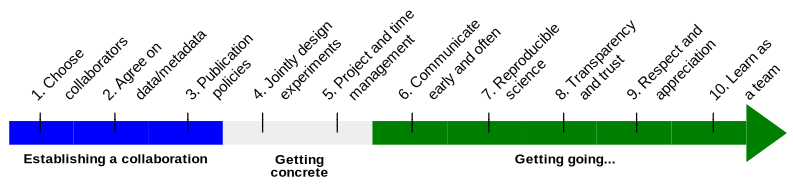
\includegraphics[width=0.99\linewidth]{timeline_linewidth_rot.pdf}}
  \caption{Typical timeline of a collaboration between experimentalists and analysts. The different steps are coarsely grouped in three phases on the timeline, but some steps are regular processes throughout the collaboration.}
  \label{fig:figure1}
\end{figure}

% \section*{Materials and methods}
% \subsection*{Etiam eget sapien nibh}

% % For figure citations, please use "Fig" instead of "Figure".
% Nulla mi mi, Fig~\ref{fig1} venenatis sed ipsum varius, volutpat euismod diam. Proin rutrum vel massa non gravida. Quisque tempor sem et dignissim rutrum. Lorem ipsum dolor sit amet, consectetur adipiscing elit. Morbi at justo vitae nulla elementum commodo eu id massa. In vitae diam ac augue semper tincidunt eu ut eros. Fusce fringilla erat porttitor lectus cursus, \nameref{S1_Video} vel sagittis arcu lobortis. Aliquam in enim semper, aliquam massa id, cursus neque. Praesent faucibus semper libero.

% % Place figure captions after the first paragraph in which they are cited.
% \begin{figure}[!h]
% \caption{{\bf Bold the figure title.}
% Figure caption text here, please use this space for the figure panel descriptions instead of using subfigure commands. A: Lorem ipsum dolor sit amet. B: Consectetur adipiscing elit.}
% \label{fig1}
% \end{figure}

% Results and Discussion can be combined.
% \section*{Results}
% Nulla mi mi, venenatis sed ipsum varius, Table~\ref{table1} volutpat euismod diam. Proin rutrum vel massa non gravida. Quisque tempor sem et dignissim rutrum. Lorem ipsum dolor sit amet, consectetur adipiscing elit. Morbi at justo vitae nulla elementum commodo eu id massa. In vitae diam ac augue semper tincidunt eu ut eros. Fusce fringilla erat porttitor lectus cursus, vel sagittis arcu lobortis. Aliquam in enim semper, aliquam massa id, cursus neque. Praesent faucibus semper libero.

% % Place tables after the first paragraph in which they are cited.
% \begin{table}[!ht]
% \begin{adjustwidth}{-2.25in}{0in} % Comment out/remove adjustwidth environment if table fits in text column.
% \centering
% \caption{
% {\bf Table caption Nulla mi mi, venenatis sed ipsum varius, volutpat euismod diam.}}
% \begin{tabular}{|l+l|l|l|l|l|l|l|}
% \hline
% \multicolumn{4}{|l|}{\bf Heading1} & \multicolumn{4}{|l|}{\bf Heading2}\\ \thickhline
% $cell1 row1$ & cell2 row 1 & cell3 row 1 & cell4 row 1 & cell5 row 1 & cell6 row 1 & cell7 row 1 & cell8 row 1\\ \hline
% $cell1 row2$ & cell2 row 2 & cell3 row 2 & cell4 row 2 & cell5 row 2 & cell6 row 2 & cell7 row 2 & cell8 row 2\\ \hline
% $cell1 row3$ & cell2 row 3 & cell3 row 3 & cell4 row 3 & cell5 row 3 & cell6 row 3 & cell7 row 3 & cell8 row 3\\ \hline
% \end{tabular}
% \begin{flushleft} Table notes Phasellus venenatis, tortor nec vestibulum mattis, massa tortor interdum felis, nec pellentesque metus tortor nec nisl. Ut ornare mauris tellus, vel dapibus arcu suscipit sed.
% \end{flushleft}
% \label{table1}
% \end{adjustwidth}
% \end{table}


% %PLOS does not support heading levels beyond the 3rd (no 4th level headings).
% \subsection*{\lorem\ and \ipsum\ nunc blandit a tortor}
% \subsubsection*{3rd level heading} 
% Maecenas convallis mauris sit amet sem ultrices gravida. Etiam eget sapien nibh. Sed ac ipsum eget enim egestas ullamcorper nec euismod ligula. Curabitur fringilla pulvinar lectus consectetur pellentesque. Quisque augue sem, tincidunt sit amet feugiat eget, ullamcorper sed velit. Sed non aliquet felis. Lorem ipsum dolor sit amet, consectetur adipiscing elit. Mauris commodo justo ac dui pretium imperdiet. Sed suscipit iaculis mi at feugiat. 

% \begin{enumerate}
% 	\item{react}
% 	\item{diffuse free particles}
% 	\item{increment time by dt and go to 1}
% \end{enumerate}


% \subsection*{Sed ac quam id nisi malesuada congue}

% Nulla mi mi, venenatis sed ipsum varius, volutpat euismod diam. Proin rutrum vel massa non gravida. Quisque tempor sem et dignissim rutrum. Lorem ipsum dolor sit amet, consectetur adipiscing elit. Morbi at justo vitae nulla elementum commodo eu id massa. In vitae diam ac augue semper tincidunt eu ut eros. Fusce fringilla erat porttitor lectus cursus, vel sagittis arcu lobortis. Aliquam in enim semper, aliquam massa id, cursus neque. Praesent faucibus semper libero.

% \begin{itemize}
% 	\item First bulleted item.
% 	\item Second bulleted item.
% 	\item Third bulleted item.
% \end{itemize}

% \section*{Discussion}
% Nulla mi mi, venenatis sed ipsum varius, Table~\ref{table1} volutpat euismod diam. Proin rutrum vel massa non gravida. Quisque tempor sem et dignissim rutrum. Lorem ipsum dolor sit amet, consectetur adipiscing elit. Morbi at justo vitae nulla elementum commodo eu id massa. In vitae diam ac augue semper tincidunt eu ut eros. Fusce fringilla erat porttitor lectus cursus, vel sagittis arcu lobortis. Aliquam in enim semper, aliquam massa id, cursus neque. Praesent faucibus semper libero~\cite{bib3}.

% \section*{Conclusion}

% CO\textsubscript{2} Maecenas convallis mauris sit amet sem ultrices gravida. Etiam eget sapien nibh. Sed ac ipsum eget enim egestas ullamcorper nec euismod ligula. Curabitur fringilla pulvinar lectus consectetur pellentesque. Quisque augue sem, tincidunt sit amet feugiat eget, ullamcorper sed velit. 

% Sed non aliquet felis. Lorem ipsum dolor sit amet, consectetur adipiscing elit. Mauris commodo justo ac dui pretium imperdiet. Sed suscipit iaculis mi at feugiat. Ut neque ipsum, luctus id lacus ut, laoreet scelerisque urna. Phasellus venenatis, tortor nec vestibulum mattis, massa tortor interdum felis, nec pellentesque metus tortor nec nisl. Ut ornare mauris tellus, vel dapibus arcu suscipit sed. Nam condimentum sem eget mollis euismod. Nullam dui urna, gravida venenatis dui et, tincidunt sodales ex. Nunc est dui, sodales sed mauris nec, auctor sagittis leo. Aliquam tincidunt, ex in facilisis elementum, libero lectus luctus est, non vulputate nisl augue at dolor. For more information, see \nameref{S1_Appendix}.


\section*{Rule 1: Choose your collaborators wisely} %%%%%%%%%%%%%%%%%%%%%%%%%%%%%%%%%%%%%%%%%%%%%%%%
\label{rule1_choose}

\begin{flushright}
\rightskip=1cm\textit{``It is better to be alone than in bad company''} \\
\vspace{.2em}
\rightskip=0cm -- George Washington
\end{flushright}

Our experience has been that good collaborators are those that are engaged not only in their own domain, but also have a thirst for knowledge about computational aspects. In many ways, this mirrors our interest in collaborative data analysis: we are tasked with handling data analysis aspects, but we endeavour to understand as much as possible of the biological context of the data. Less attractive collaborators are those that simply want a table of P-values or a set of figures; worst-case scenario are those that perceive that we simply press a button to do so. 

Choosing collaborators represents the first fundamental step for collaboration between wet-lab and dry-lab researchers. In particular, we suggest to carefully discuss scientific interests and values with potential collaborators; discrepancies are harder to navigate later on. Two questions should be considered. First, is there an adequate scientific match in the collaboration (e.g., for us, analysis of a certain type of omic data)? That is, do the groups complement each other well in terms of scientific interests and skills? Second, are (research) values between groups aligned? Meaning, do both groups have broadly similar ideas of how research is to be conducted day-to-day? For example, is excellence defined as a Cell/Nature/Science paper, or is it robust and high quality science?

In practice, collaborations originate between researchers who know each other already (e.g., in the same institute). Thus, the scientific match is usually there or can be easily established. Ascertaining the alignment of research values is more difficult and sometimes requires months and years of working together to fully comprehend. 

In addition, choosing collaborators can also be thought of as a process that repeats itself at natural stopping points, such as the finishing of a project (stage). It can be advantageous to evaluate at regular intervals whether all parties are getting what they had hoped out of the collaboration and re-discuss the collaboration if not.

In our experience, most friction arises from having different expectations that are not clearly expressed nor negotiated. To detect and smoothen possible misalignments (for this and other rules) we suggest both teams fill an expectations form (such as \nameref{S1_table}), compare them, and discuss conflicting views early on. Explicit is better than implicit. 

Actionable items: openly discuss expectations (\nameref{S1_table}); be transparent and agree on funding sources (i.e. ideologically loaded private foundations).

\section*{Rule 2: Agree on data and metadata structure} %%%%%%%%%%%%%%%%%%%%%%%%%%%%%%%%%%%%%%%%%%
\label{rule2_data}

\begin{flushright}
\rightskip=1cm\textit{``With big data comes big responsibilities''} \\
\vspace{.2em}
\rightskip=0cm -- Kate Crawford
\end{flushright}

In omics data analysis, there are typically many stages to an analysis, each one having its own type of data (e.g., raw data, filtered data, normalized data, modelling, inference, etc). How and what data are shared internally between the project members during the project should be agreed upon, i.e how are data shared between collaborators, what (intermediate) data can be shared, data formats that can be easily read by all researchers. The FAIR principles \cite{wilkinson2016fair} on data sharing offer good guidelines and can be useful later when publishing the open data of the project.

Sensitive data (frequently patient-related personal data) represent a special case as they require additional protection with data storage and sharing.  A data sharing agreement should be determined between the collaborators. Analysts working on these datasets are obliged to take steps in accordance with the law and the signed agreement. Normally the agreement specifies who is granted access to the data; the purpose of the data analysis; what measures need to be taken (e.g., access, logging) to ensure the privacy and integrity of the data. 

Clear standards for metadata format and style are often lacking (even among some fields of computer science), which can often lead to misleading or erroneous data and ultimately to biased results. A good practice is to agree on a common and systematic way of sharing the metadata, which can both be easily accessible and modified by experimentalists, and easily parsed by analysts, and consistent enough to be integrated in an analysis workflow.  

Actionable items: Follow the FAIR guidelines (\url{https://www.go-fair.org/fair-principles/}); define file naming policies; be aware of sensitive data handling regulations in your country (e.g. GDPR in Europe \cite{shabani2019reidentifiability,party2011advice}, PIPEDA in Canada \cite{phillips2018international}, HIPAA in the US \cite{phillips2018international}); follow good practices for spreadsheets \cite{broman2018data}.

\section*{Rule 3: Define publication policies} %%%%%%%%%%%%%%%%%%%%%%%%%%%%%%%%%%%%%%%%%%%%%%%%%%%%
\label{rule3_publication}

\begin{flushright}
\rightskip=1cm\textit{``The only good ideas are the ones I can take credit for''} \\
\vspace{.2em}
\rightskip=0cm -- Richard Stevens
\end{flushright}

Explicitly ask your collaborator's expectations on research dissemination, openly express yours and reach consensus. Expectations to discuss include strategies on paper publishing, conferences, and other deliverables, such as software; in particular, basic ground rules for author ordering should be broached.

For academic papers, discuss potential target and no-go journals, (posting and updating) preprints, and open access. For other deliverables, particularly software and data analysis workflows, discuss intellectual property, copyright, open software licenses, and whether these deliverables can be disseminated independently of the main collaboration paper or not. A common model that our research group accomplishes is two manuscripts: one primarily biological where we are second and second-last authors; and the other primarily methodological, where we are first and last authors.

Discuss author order expectations early, particularly for first author, senior and corresponding roles. Also consider co-contributions, co-correspondence, and flexibility for future updates (i.e., new people joining the team). Do not neglect the ordering within co-authors, if applicable. Be aware of possible sources of biases during this negotiation, including gender, PI's favouritism, seniority or tradition (i.e., wet labs taking precedence over dry lab). The same considerations apply to senior and corresponding authors. 

Actionable items: Embrace author contribution taxonomies like CRediT \cite{allen2014publishing} (\url{https://credit.niso.org/}), re-evaluate the policy in case of major change of contributions or because of new collaborators joining while the project is ongoing.

\section*{Rule 4: Jointly design the experiments} %%%%%%%%%%%%%%%%%%%%%%%%%%%%%%%%%%%%%%%%%%%%%%%%%
\label{rule4_experiments}

%\begin{flushright}
%\rightskip=1cm\textit{``To consult the statistician after an experiment is finished is often merely to ask [$\ldots$] to conduct a post-mortem examination [$\ldots$] [and] perhaps say what the experiment died of''} \\
%\vspace{.2em}
%\rightskip=0cm -- Ronald A. Fisher
%\end{flushright}

\begin{flushright}
\rightskip=1cm\textit{``No one believes an hypothesis except its originator but everyone believes an experiment except the~experimenter''} \\
\vspace{.2em}
\rightskip=0cm -- William Ian Beardmore Beveridge
\end{flushright}

Under experimental design, we are referring to the process of defining the general workflow to reach a certain outcome such as testing a hypothesis, answering a biological question or demonstrating a new experimental assay. This encompasses primarily the wet lab experiments but can also include data analysis. Ideally, the project members would define the core aspects of the experimental design prior to collecting data. As a first step, the goal of the research project should be clearly formulated and agreed upon. Both teams should then be involved in the definition of all steps of the experimental design. This may happen at different levels depending on their area of expertise, but all members should have a basic knowledge on all steps of the workflow, including wet lab and dry lab. After defining the experimental design, you should agree with your collaborators on a rough analysis plan. After defining the main steps of the experimental design and analysis plan, a rough timeline should also be generated (see also \nameref{rule5_time}). Finally, the minimal desired outcome (such as initial data analysis, final figures, etc) should also be defined. 

The agreed-upon timeline may be reevaluated after obtaining the initial results. In this case, any changes in the experimental design and/or analysis should be discussed and agreed upon by members of both the wet lab and dry lab. 

Often, dry labs are approached by wet labs to initiate a collaboration (see \nameref{rule1_choose}) after the research question has already been defined and initial wet lab experiments have been performed (and sometimes after primary bioinformatics analysis has been conducted). Starting a collaboration at this stage is often risky and harder than being engaged from the start of the project, since strong expectations for the project may already be set by the wet lab researchers. You should then evaluate whether the proposition from the wet lab users makes sense. If needed, they should suggest additional controls / experiments that would be helpful for downstream data analysis or to reach the final aim of the project.

Actionable items: include test and pilot experiments in your experimental design.

\section*{Rule 5: Agree on project and time management} %%%%%%%%%%%%%%%%%%%%%%%%%%%%%%%%%%%%%%%%%%%%
\label{rule5_time}

\begin{flushright}
\rightskip=1cm\textit{``If it's your job to eat a frog, it's best to do it first thing in the morning. And If it's your job to eat two frogs, it's best to eat the biggest one first''} \\
\vspace{.2em}
\rightskip=0cm -- Mark Twain
\end{flushright}

Define together individual tasks and responsibilities, the days or working hours allocated to that project (for communication and urgent tasks to perform), as well as time horizons (in calendar months) for these and for the collaboration more generally. This is also important to get a grasp of the complexity of tasks beyond your expertise that one might underestimate. Plan with buffer time for unforeseen complications. Explicitly check your expectations are aligned (\nameref{S1_table}).

To ensure mutual awareness and help monitor progress, it can be useful to keep an up-to-date project plan where everyone can see what was done and what is currently being worked on by whom. If there are digressions or changes of plan, discuss them with the collaborators ahead of engaging in many hours of work. Since most people involved will also have a number of other engagements (and holidays!) with loads that vary over time, it is important to inform each other, ahead of time if possible, of the varying availability for collaboration. Regular meetings, either planned or in response to new data or emerging problems, are also critical to a smooth collaboration (see \nameref{rule6_communication}). 

Actionable items: use online project planners (i.e., Trello, GitHub projects, etc); use multiuser online text editors (i.e., Google Docs, Overleaf) to draft manuscripts and other documents.

\section*{Rule 6: Communicate early, openly, and often enough} %%%%%%%%%%%%%%%%%%%%%%%%%%%%%%%%%%%%%%%%
\label{rule6_communication}

\begin{flushright}
\rightskip=1cm\textit{``The single biggest problem in communication is the illusion that it has taken place''} \\
\vspace{.2em}
\rightskip=0cm -- George Bernard Shaw
\end{flushright}

Establishing a productive and respectful communication strategy is essential for fruitful and low-friction collaborations. To ensure clarity, a mutual expectation agreement is also needed regarding project length, cost sharing, preferred communication channels and frequency, as well as expected response times. Regular meetings, prompt feedback (for a mutually-agreed definition of prompt), and attending relevant meetings all help maintain alignment on communication. Communication should not only take place when you need something concrete from your collaborators, but sharing and feedback require continuous cycling. However, all collaborators should be empathetic and flexible in meeting plans or project progress due to other responsibilities (teaching duties, other projects, personal reasons) and with mutual respect to others’ work hours (see \nameref{rule5_time}). Especially after long or complicated discussions, or when multiple people were involved, it can be helpful to prepare a summary of important discussion points and decisions to be circulated in written form (e.g., Google Docs or via a Slack or Mattermost channel), to represent a common understanding and have a memento of the conversations.

Actionable items: Adhere to effective meetings \cite{leblanc2019planning} and written interactions guidelines \cite{gruber2020email}.

\section*{Rule 7: Follow open and reproducible science guidelines} %%%%%%%%%%%%%%%%
\label{rule7_repro}

\begin{flushright}
\rightskip=1cm\textit{``The way of the world is to make laws, but follow custom''} \\
\vspace{.2em}
\rightskip=0cm -- Michel de Montaigne
\end{flushright}

Project members should follow reproducible research practices (e.g., use FAIR file formats, version control, free and open source software, good coding practices and reproducible reporting \cite{wilkinson2016fair,sandve2013ten,stawarczyk2023establishing} to ensure that data analysis is transparent and everyone can recreate your results and findings. Before a project starts, agree on the desired degree of public data availability (see also \nameref{rule2_data}) and how (and if) to report summary statistics of sensitive data. Typically, journal policies require authors to describe their data and code availability; this leaves room to share anything from raw data to intermediate results, as well as unstructured code to analysis reports to fully reproducible pipelines. Make sure your collaborators agree with your high commitment to transparency and reproducibility. As a project goes on, it becomes increasingly important to keep all data, software environments, online code, and reports tractable. Ensuring code and results (figures and tables) are in accessible states and versioned enables everyone to stay updated on discussions, failed attempts, and outcomes. Similarly, literate programming \cite{knuth1984literate}, e.g., generating reports with both code and results in open formats (HTML, PDF), facilitates scientific reproducibility and open access. Reproducible computational research is crucial for guaranteeing the consistency and transparency of scientific discoveries. Conversely, a lack of reproducibility threatens all findings.

Since the expertise of both sides differ, it is important to agree on an adequate strategy for sharing results and adapt it to expectations and technical abilities. Although sharing the code among analysts is (or should be) a standard, reports shared with experimentalists could be easier to digest when limited to figures, main results and conclusions. The format to share results should also be clearly defined (meetings, static reports, dynamic reports, etc) and always discussed between the two parts to promote a clear understanding of the collaboration's outputs.   

Actionable items: use version control (git) and push frequently to remotes shared with your collaborators (i.e., GitHub, BitBucket, GitLab); include reproducible and versioned software installation steps in your code repositories; create an analysis workflow that can easily be rerun after a change in the data or in the analysis.

\section*{Rule 8: Establish the transparency and trust required for constructive feedback} %%%%%%%%%
\label{rule8_trust}

\begin{flushright}
\rightskip=1cm\textit{``Far better an approximate answer to the right question, which is often vague, than an exact answer to the wrong question, which can always be made precise''} \\
\vspace{.2em}
\rightskip=0cm -- John Tukey
\end{flushright}

Project teams should jointly engage in thorough sanity checks throughout the research. This involves regularly questioning and testing various aspects of the project, in both wet and dry lab domains (see~\nameref{rule7_repro}). It might include repeating experiments to confirm their consistency, and using different analysis approaches to explore robustness of results to analysis choices. Both sides should be transparent about the specifics and the output of their work, including unsuccessful attempts, failed controls, irreproducible or not-straightforward-to-interpret results. The reporting of unsuccessful results not only helps to build trust and transparency between both sides, but also helps to discuss alternatives and improve the (wet lab or dry lab) process. Results should be shared fully, e.g., raw western blots, raw imaging data, and all quality control checks. The goal of such a continuous policy of critical thinking and sanity checking is to maintain integrity and build trust among collaborators; and to confirm that both the experimental setups and computational analyses are functioning as expected. By routinely challenging the integrity and interpretability of wet lab and analysis results, potential misalignments can be avoided.

Actionable items: share all raw and processed data; listen to and acknowledge dissenting opinions.

\section*{Rule 9: Be respectful and show appreciation} %%%%%%%%%%%%%%%%%%%%%%%%%%%%%%%%%%%%%%%%%%%
\label{rule9_respect}

\begin{flushright}
\rightskip=1cm\textit{``By mutual confidence and mutual aid great deeds are done, and great discoveries made''} \\
\vspace{.2em}
\rightskip=0cm -- Homer
\end{flushright}

Acknowledge that everyone who has agreed to take part in the collaboration has their validity and represents a different aspect of the scientific endeavour. There is no role that is \textit{per se} more important than the others, no matter how niche it is. Mutual respect of each other’s work and (domain-specific) knowledge should be a given. In turn, this does not rule out but rather includes the questioning and critical assessment of each other's results on a scientific level in case of doubt (see~\nameref{rule8_trust}). Limitations of both scientific approaches but also personal availability for the project should be clearly stated and respected by the other parties involved (see \nameref{rule6_communication}). Polite communication between collaborators is required at all times, be it when discussing potentially unsatisfying results or agreeing on a time schedule for future steps. Be kind: do not forget to regularly acknowledge and thank others for their work, and explicitly remind you and others the project could not be carried out alone.

Actionable items: be respectful; be aware of common cognitive biases, including the impostor syndrome \cite{clance1978imposter} and Dunning–Kruger effect \cite{kruger1999unskilled}.

\section*{Rule 10: Learn as a team} %%%%%%%%%%%%%%%%%%%%%%%%%%%%%%%%%%%%%%%%%%%%%%%%%%%%%%%%%%%%%%%
\label{rule10_learn}

\begin{flushright}
\rightskip=1cm\textit{``Question everything. Learn something. Answer nothing''} \\
\vspace{.2em}
\rightskip=0cm -- Euripides 
\end{flushright}

The more you know about what the other side is doing and why, the easier the collaboration. It is of great help if everyone involved has both a basic understanding of the different experimental and computational components involved as well as the willingness to gain a deeper understanding of each others methodology as the collaboration proceeds. What can we really interpret from a PCA plot or how does the library preparation protocol influence sequencing results? This common knowledge is not a requirement at the start of a collaboration but can be established during the project. Treat knowledge gaps as an opportunity to learn something new. This should be practised at all levels, irrespective of level of seniority. It will make the common work and communication a lot easier. For example, it will save the analyst a lot of time if the metadata are machine-readable, in turn a wet-lab collaborator might gain more independence if the analysis scripts and outputs are easily accessible to them and well documented. Take advantage of the diversity of backgrounds as it provides different perspectives on a problem that can offer new approaches to solve problems.

Actionable items: add explanatory comments to the analysis code; do not shy away from asking what you do not understand; commit to answering basic and advanced questions about the analysis.

\section*{Conclusion} %%%%%%%%%%%%%%%%%%%%%%%%%%%%%%%%%%%%%%%%%%%%%%%%%%%%%%%%%%%%%%%%%%%%%%%%%%%%%%

In any situation when multiple (scientific) cultures collide, there can be tension and misunderstandings at some stage and there is no simple formula to navigate all the personalities and egos involved. Let us not forget that along the way, all members of a collaboration need to absorb a vast assortment of private as well as work pressures, power differentials, deadlines and commitments. Nonetheless, these differences and cultural quirks are a reality to be observed, studied and understood such that we can embrace the diversity of scientific mindsets. We also note that the goal is not necessarily to pursue fully harmonious collaborations, because stumbling through our misunderstandings helps us crystalize norms for collaborations and define our core values of doing science. This may lead to lifelong collaborations or also to those that will never happen again.

Collaborative data analysis is not our primary role, but in many cases becomes the springboard to new methodological projects. The ten simple tips discussed here are largely about being open, organized, empathetic, professional, practical, systematic, and fair.


\section*{Supporting information}

% Include only the SI item label in the paragraph heading. Use the \nameref{label} command to cite SI items in the text.
% \paragraph*{S1 Fig.}
% \label{S1_Fig}
% {\bf Bold the title sentence.} Add descriptive text after the title of the item (optional).

% \paragraph*{S2 Fig.}
% \label{S2_Fig}
% {\bf Lorem ipsum.} Maecenas convallis mauris sit amet sem ultrices gravida. Etiam eget sapien nibh. Sed ac ipsum eget enim egestas ullamcorper nec euismod ligula. Curabitur fringilla pulvinar lectus consectetur pellentesque.

\paragraph*{S1 Table.}
\label{S1_table}
{\bf Collaboration expectations form.} The idea here is that there are no good answers (well, sometimes there are), but that each party fills the form and then compares their answer, to hopefully align expectations. Some questions are phrased rhetorically, but meant to explicitly prepare all members for a collaboration's potential tension points. To fill put an `x' in the appropriate column, where 3 is `agree equally with both statements', 1 is `strongly agree with statement on left', and 5 is `strongly agree with statement on right'.

% \paragraph*{S1 Video.}
% \label{S1_Video}
% {\bf Lorem ipsum.}  Maecenas convallis mauris sit amet sem ultrices gravida. Etiam eget sapien nibh. Sed ac ipsum eget enim egestas ullamcorper nec euismod ligula. Curabitur fringilla pulvinar lectus consectetur pellentesque.

% \paragraph*{S1 Appendix.}
% \label{S1_Appendix}
% {\bf Lorem ipsum.} Maecenas convallis mauris sit amet sem ultrices gravida. Etiam eget sapien nibh. Sed ac ipsum eget enim egestas ullamcorper nec euismod ligula. Curabitur fringilla pulvinar lectus consectetur pellentesque.

% \paragraph*{S1 Table.}
% \label{S1_Table}
% {\bf Lorem ipsum.} Maecenas convallis mauris sit amet sem ultrices gravida. Etiam eget sapien nibh. Sed ac ipsum eget enim egestas ullamcorper nec euismod ligula. Curabitur fringilla pulvinar lectus consectetur pellentesque.

\section*{Acknowledgments}
We thank our past collaborators for their often-pleasurable, sometimes-painful contributions that led to to distilling these rules.

The content of this manuscript was brainstormed during a lab retreat in the scenic town of Aeschi bei Spiez, Switzerland.

\nolinenumbers

% Either type in your references using
% \begin{thebibliography}{}
% \bibitem{}
% Text
% \end{thebibliography}
%
% or
%
% Compile your BiBTeX database using our plos2015.bst
% style file and paste the contents of your .bbl file
% here. See http://journals.plos.org/plosone/s/latex for 
% step-by-step instructions.
%


% \bibliography{ten_simple_rules_collaborations_2024}

% \begin{thebibliography}{10}

% \bibitem{bib1}
% Conant GC, Wolfe KH.
% \newblock {{T}urning a hobby into a job: how duplicated genes find new
%   functions}.
% \newblock Nat Rev Genet. 2008 Dec;9(12):938--950.

% \bibitem{bib2}
% Ohno S.
% \newblock Evolution by gene duplication.
% \newblock London: George Alien \& Unwin Ltd. Berlin, Heidelberg and New York:
%   Springer-Verlag.; 1970.

% \bibitem{bib3}
% Magwire MM, Bayer F, Webster CL, Cao C, Jiggins FM.
% \newblock {{S}uccessive increases in the resistance of {D}rosophila to viral
%   infection through a transposon insertion followed by a {D}uplication}.
% \newblock PLoS Genet. 2011 Oct;7(10):e1002337.

\begin{thebibliography}{10}

\bibitem{cechova2020ten}
  Cechova M.
\newblock Ten simple rules for biologists initiating a collaboration with
computer scientists.
\newblock PLoS Computational Biology. 2020;16(10):e1008281.

\bibitem{aron2021ten}
Aron S, Jongeneel CV, Chauke PA, Chaouch M, Kumuthini J, Zass L, et~al..
\newblock Ten simple rules for developing bioinformatics capacity at an academic
  institution.
\newblock PLoS Computational Biology. 2021;17(12):e1009592.

\bibitem{knapp2015ten}
Knapp B, Bardenet R, Bernabeu MO, Bordas R, Bruna M, Calderhead B, et~al.. 
  \newblock Ten
  simple rules for a successful cross-disciplinary collaboration.
  \newblock PLoS Computational Biology, 2015;11(4):e1004214.
  
\bibitem{kumuthini2020ten}
Kumuthini J, Chimenti M, Nahnsen S, Peltzer A, Meraba R, McFadyen R, et~al..
  \newblock Ten simple rules for providing effective bioinformatics research support.
  \newblock PLoS computational biology. 2020;16(3):e1007531.
  
\bibitem{wilkinson2016fair}
Wilkinson MD, Dumontier M, Aalbersberg IJ, Appleton G, Axton M, Baak A, et~al.
\newblock The FAIR Guiding Principles for scientific data management and
  stewardship.
\newblock Scientific Data. 2016;3(1):160018.
\newblock doi:{10.1038/sdata.2016.18}.

\bibitem{shabani2019reidentifiability}
Shabani M, Marelli L.
\newblock Re-identifiability of genomic data and the GDPR: Assessing the
  re-identifiability of genomic data in light of the EU General Data Protection
  Regulation.
\newblock EMBO reports. 2019;20(6):e48316.

\bibitem{party2011advice}
{Data~Protection~Working~Party}.
\newblock Advice paper on special categories of data (“sensitive data”).
\newblock Article 29 of Directive 95/46/EC, Ares 444105. 2011;.

\bibitem{phillips2018international}
Phillips M.
\newblock International data-sharing norms: from the OECD to the General Data
  Protection Regulation (GDPR).
\newblock Human genetics. 2018;137:575--582.

\bibitem{broman2018data}
Broman KW, Woo KH.
\newblock Data organization in spreadsheets.
\newblock The American Statistician. 2018;72(1):2--10.

\bibitem{allen2014publishing}
Allen L, Scott J, Brand A, Hlava M, Altman M.
\newblock Publishing: Credit where credit is due.
\newblock Nature. 2014;508(7496):312--313.

\bibitem{leblanc2019planning}
LeBlanc LA, Nosik MR.
\newblock Planning and leading effective meetings.
\newblock Behavior Analysis in Practice. 2019;12(3):696--708.

\bibitem{gruber2020email}
Gruber J, H SL, van Bavel JJ. A scientist's guide to email etiquette; 2020.
\newblock Available from:
  \url{http://doi.org/10.1126/science.caredit.abb2664}.

\bibitem{sandve2013ten}
Sandve GK, Nekrutenko A, Taylor J, Hovig E.
\newblock Ten simple rules for reproducible computational research.
\newblock PLoS Computational Biology. 2013;9(10):e1003285.

\bibitem{stawarczyk2023establishing}
Stawarczyk B, Roos M.
\newblock Establishing effective cross-disciplinary collaboration: Combining
  simple rules for reproducible computational research, a good data management
  plan, and good research practice.
\newblock PLoS Computational Biology. 2023;19(4):e1011052.

\bibitem{knuth1984literate}
Knuth DE.
\newblock Literate programming.
\newblock The computer journal. 1984;27(2):97--111.

\bibitem{clance1978imposter}
Clance PR, Imes SA.
\newblock The imposter phenomenon in high achieving women: Dynamics and
  therapeutic intervention.
\newblock Psychotherapy: Theory, research \& practice. 1978;15(3):241.

\bibitem{kruger1999unskilled}
Kruger J, Dunning D.
\newblock Unskilled and unaware of it: how difficulties in recognizing one's
  own incompetence lead to inflated self-assessments.
\newblock Journal of personality and social psychology. 1999;77(6):1121.

\end{thebibliography}



\end{document}

